\subsection{Verification of non-linear model}
In this section the results from simulation of the equation of movement in \autoref{eq:thetaForce} is presented and compared with test results describing the movement of the segway. This is done to clarify the difference between the non-linear model and the reality it describes.
\subsubsection{Simulation in Simulink}\label{subsec:SiS}
A block diagram is compiled from \autoref{eq:thetaForce}, the block diagram is shown in \autoref{fig:nonLinBlock}. All simulated data in \autoref{subsec:CSR} is from this block diagram.
The sample rate and total simulation time is the same as the ones for the data acquisition from the test. Since there is a delay in the test data acquisition, before the inverted pendulum is released, this delay has also been included in the discrete impulse used in the simulation.
\todo{Write something about the damper value, how it has been, or should be determined (In fig it is 3)}
\begin{figure}[H]
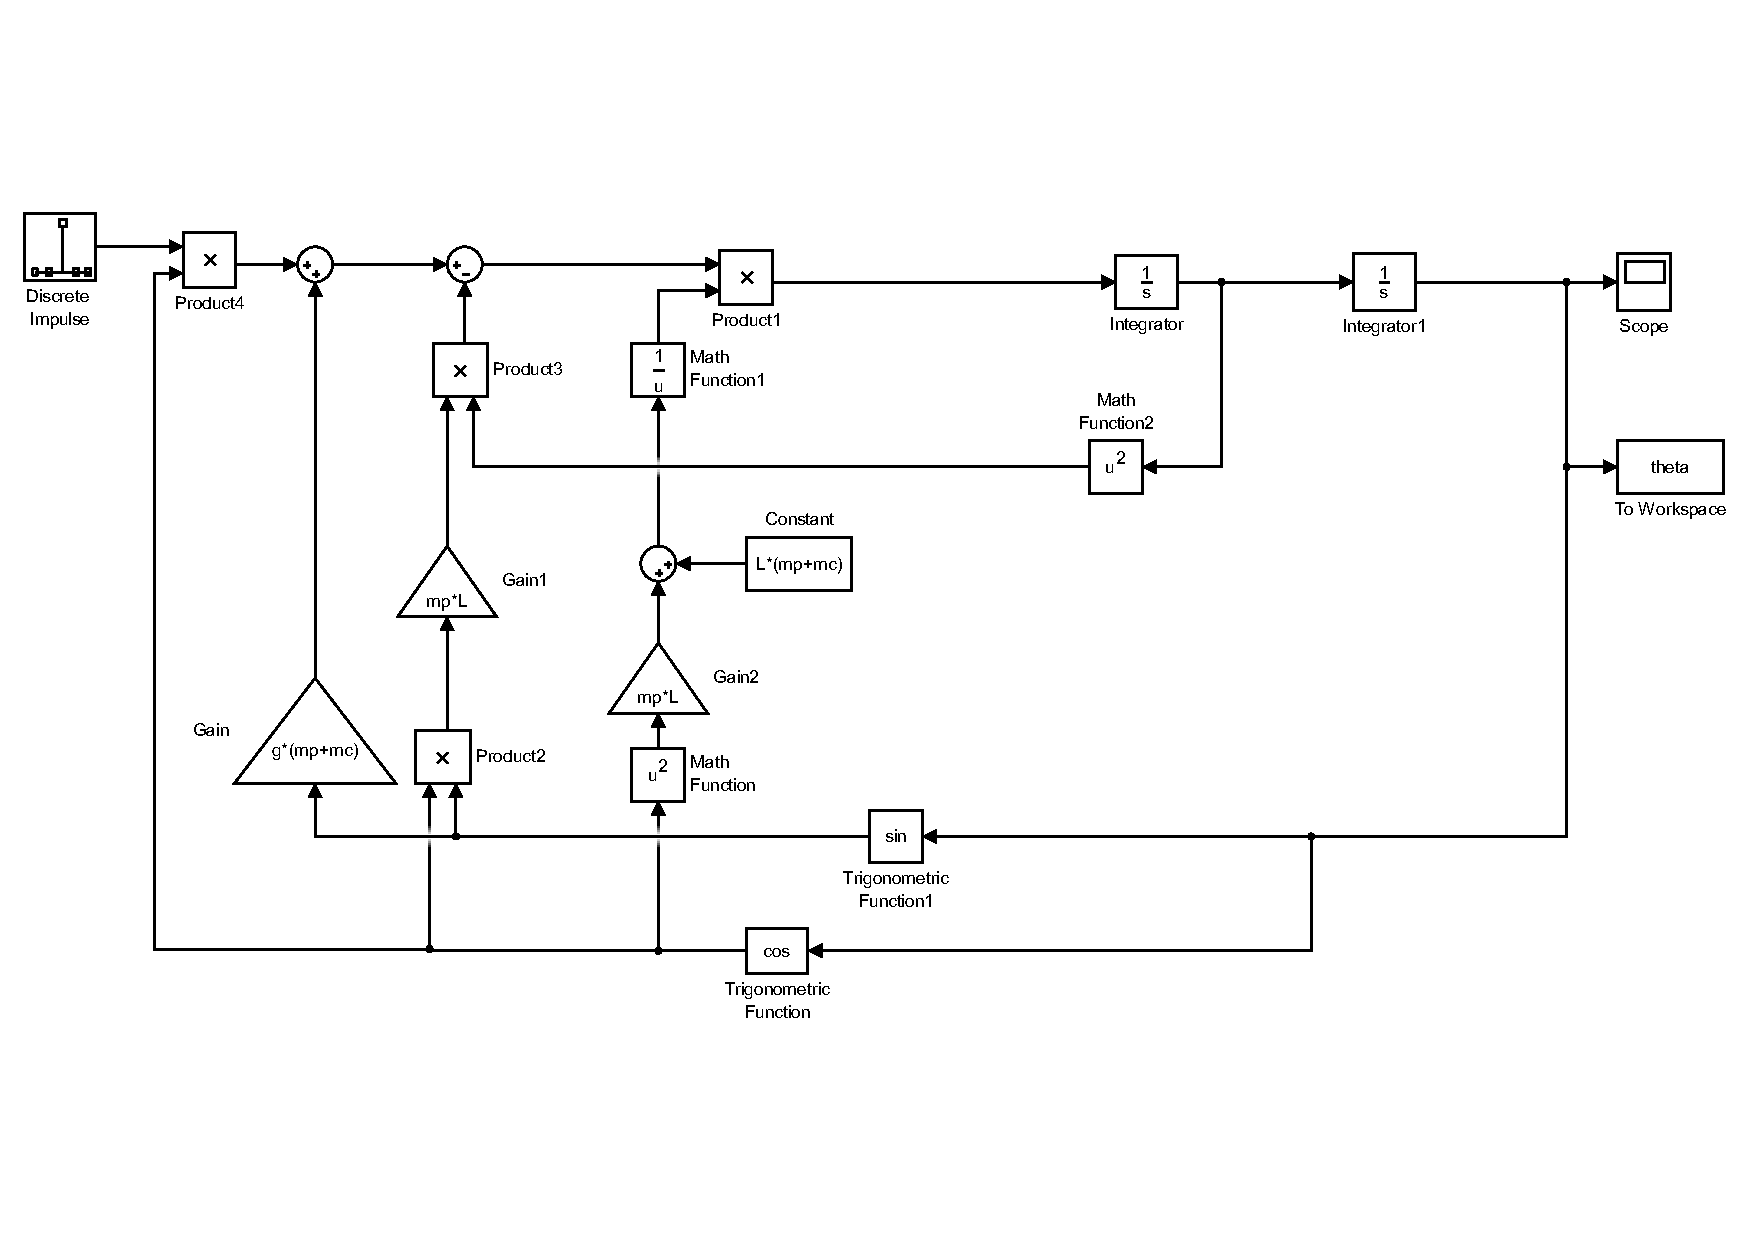
\includegraphics[width=\textwidth]{figures/BlockIPNL.pdf}
\caption{Block diagram of the non-linear inverted pendulum.\label{fig:nonLinBlock}}
\end{figure}






\subsubsection{Comparison between simulation and test}\label{subsec:CSR}
The test of the segway, has been performed as it is written in \autoref{App:viconNonLin} and the simulation as described in \autoref{subsec:SiS}. The simulated data and the data from the test can be seen in the figures: \ref{fig:comThetaBig}, \ref{fig:comThetaSmall} and \ref{fig:comPos}.
\todo{Write a measurement report about the vicon data acquisition for the non-linear model.}
\begin{figure}
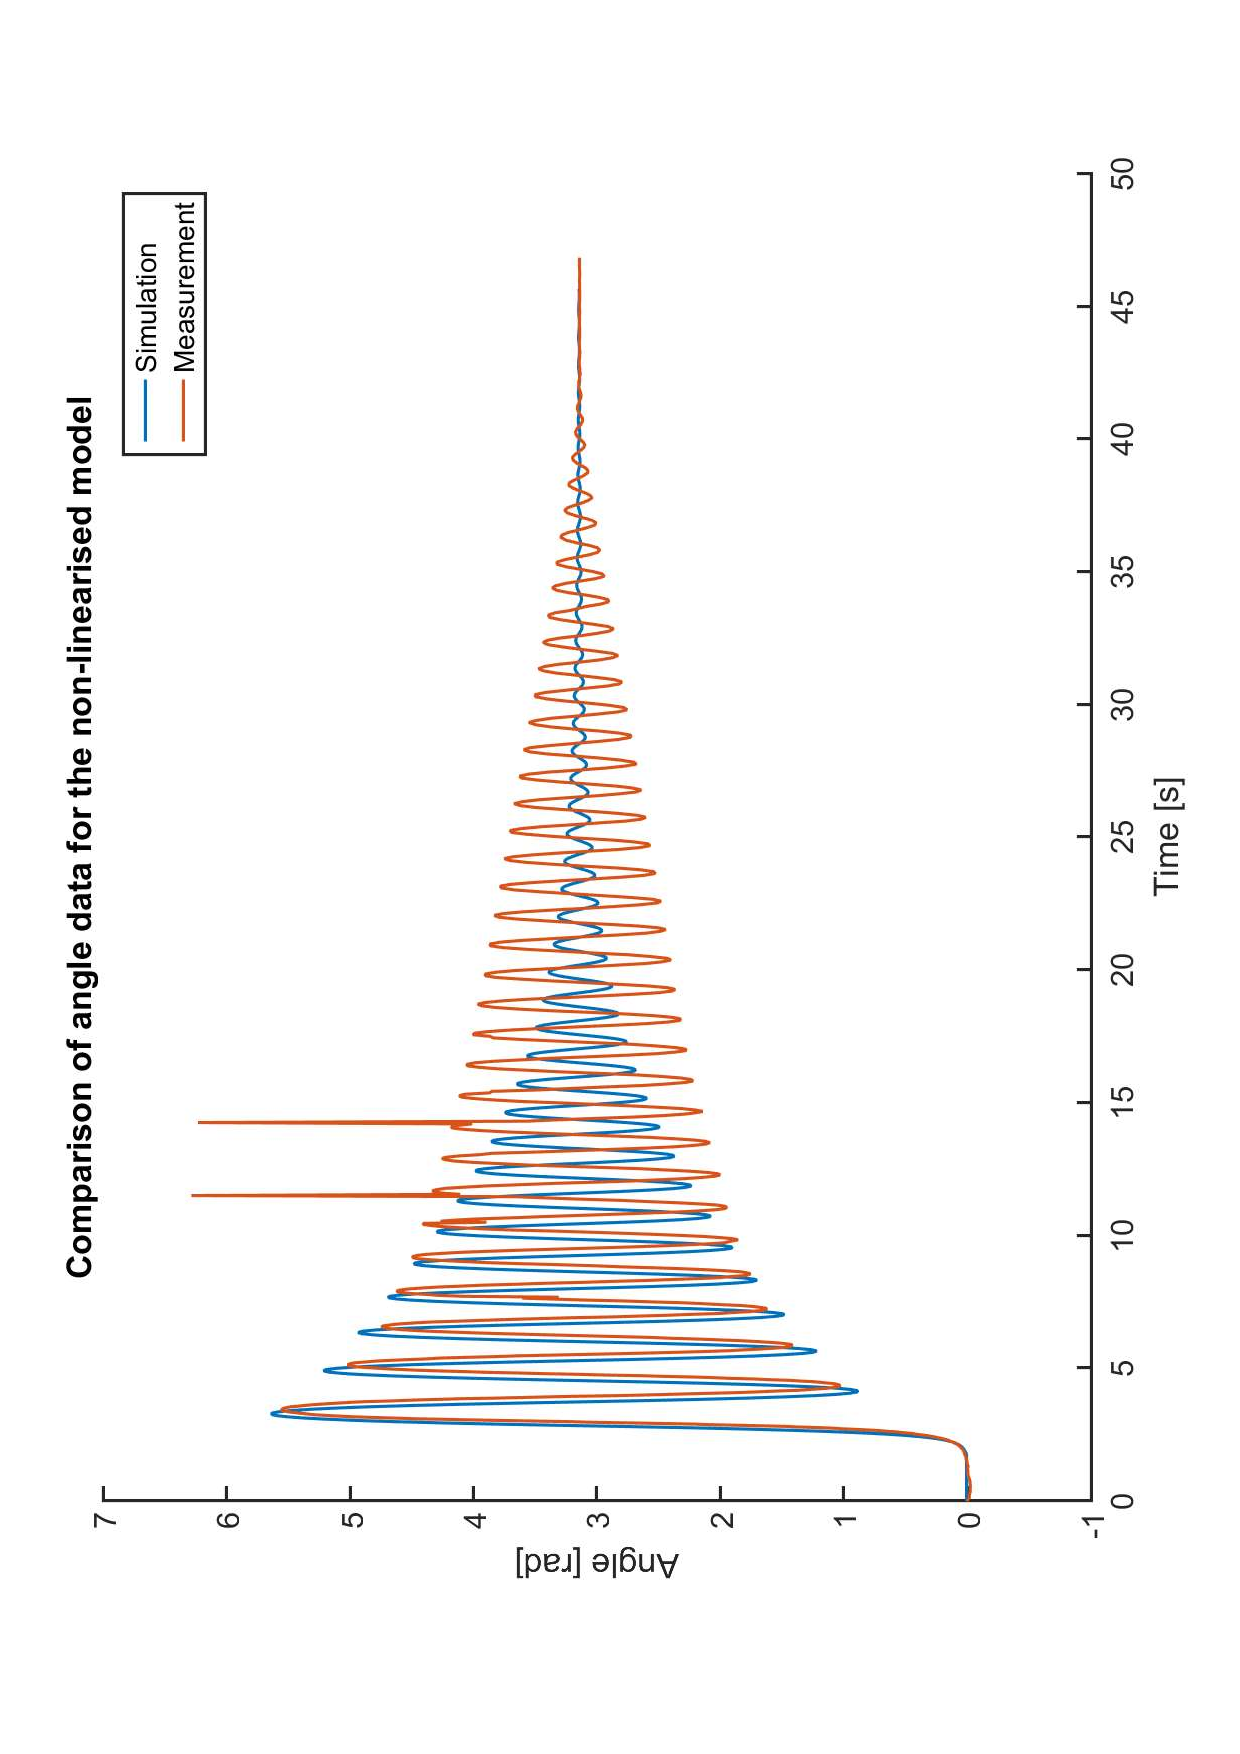
\includegraphics[height=\textwidth, angle = -90]{figures/SimMesInvPenThetaBig.pdf}
\caption{Graph showing the entire impulse response of $\theta$ for the simulation and the test. The two spikes are glitches. \label{fig:comThetaBig}}
\end{figure}
The graph in \autoref{fig:comThetaBig} shows that there is a close relation between the two impulse responses for the first few oscillations of the pendulum. Unfortunately, this close relation doesn't continue, as the measured oscillation, becomes more linear in its damping and the period decreases. Both of these attributes are not expected of an ideal inverted pendulum, and is likely caused by dry friction and stiction. On the other hand it may also be caused by the rails the segway stood on were not immovable.

Since the segway will be standing on a surface, it will not be able to rotate more than $90\deg$ in either direction, thus the most important part of the comparison is the one from 0 to $\frac{\pi}{2}$ radians. This part of the comparison is shown in \autoref{fig:comThetaSmall}.
\begin{figure}
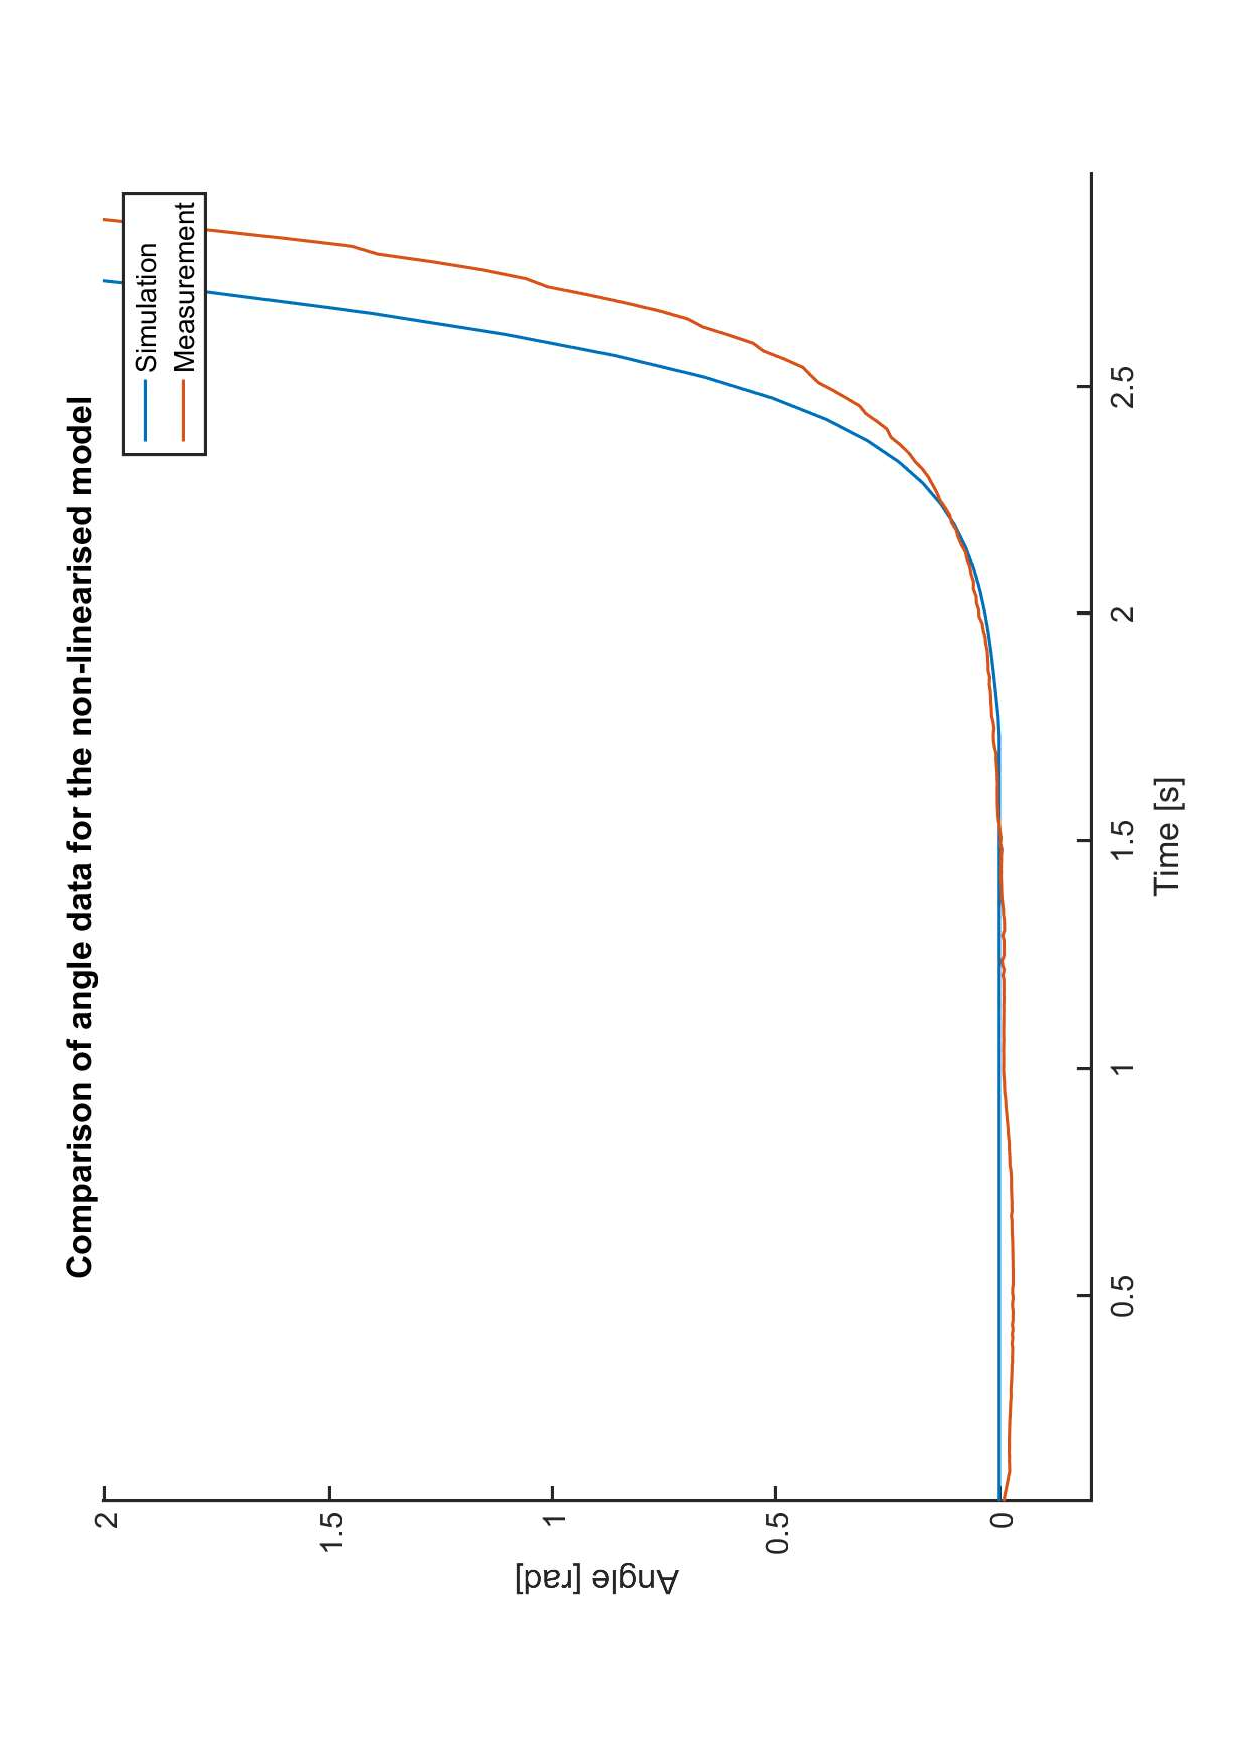
\includegraphics[height=\textwidth, angle = -90]{figures/SimMesInvPenThetaSmall.pdf}
\caption{Graph showing the first few radians of the impulse response for $\theta$ for the simulation and the test.\label{fig:comThetaSmall}}
\end{figure}
From the graph in \autoref{fig:comThetaSmall} it is seen that the simulation and test results are closely related, especially for small angles. For larger angles, the response time of the model is faster than that of the reality. This is likely due to the before mentioned dry friction and stiction.

\begin{figure}
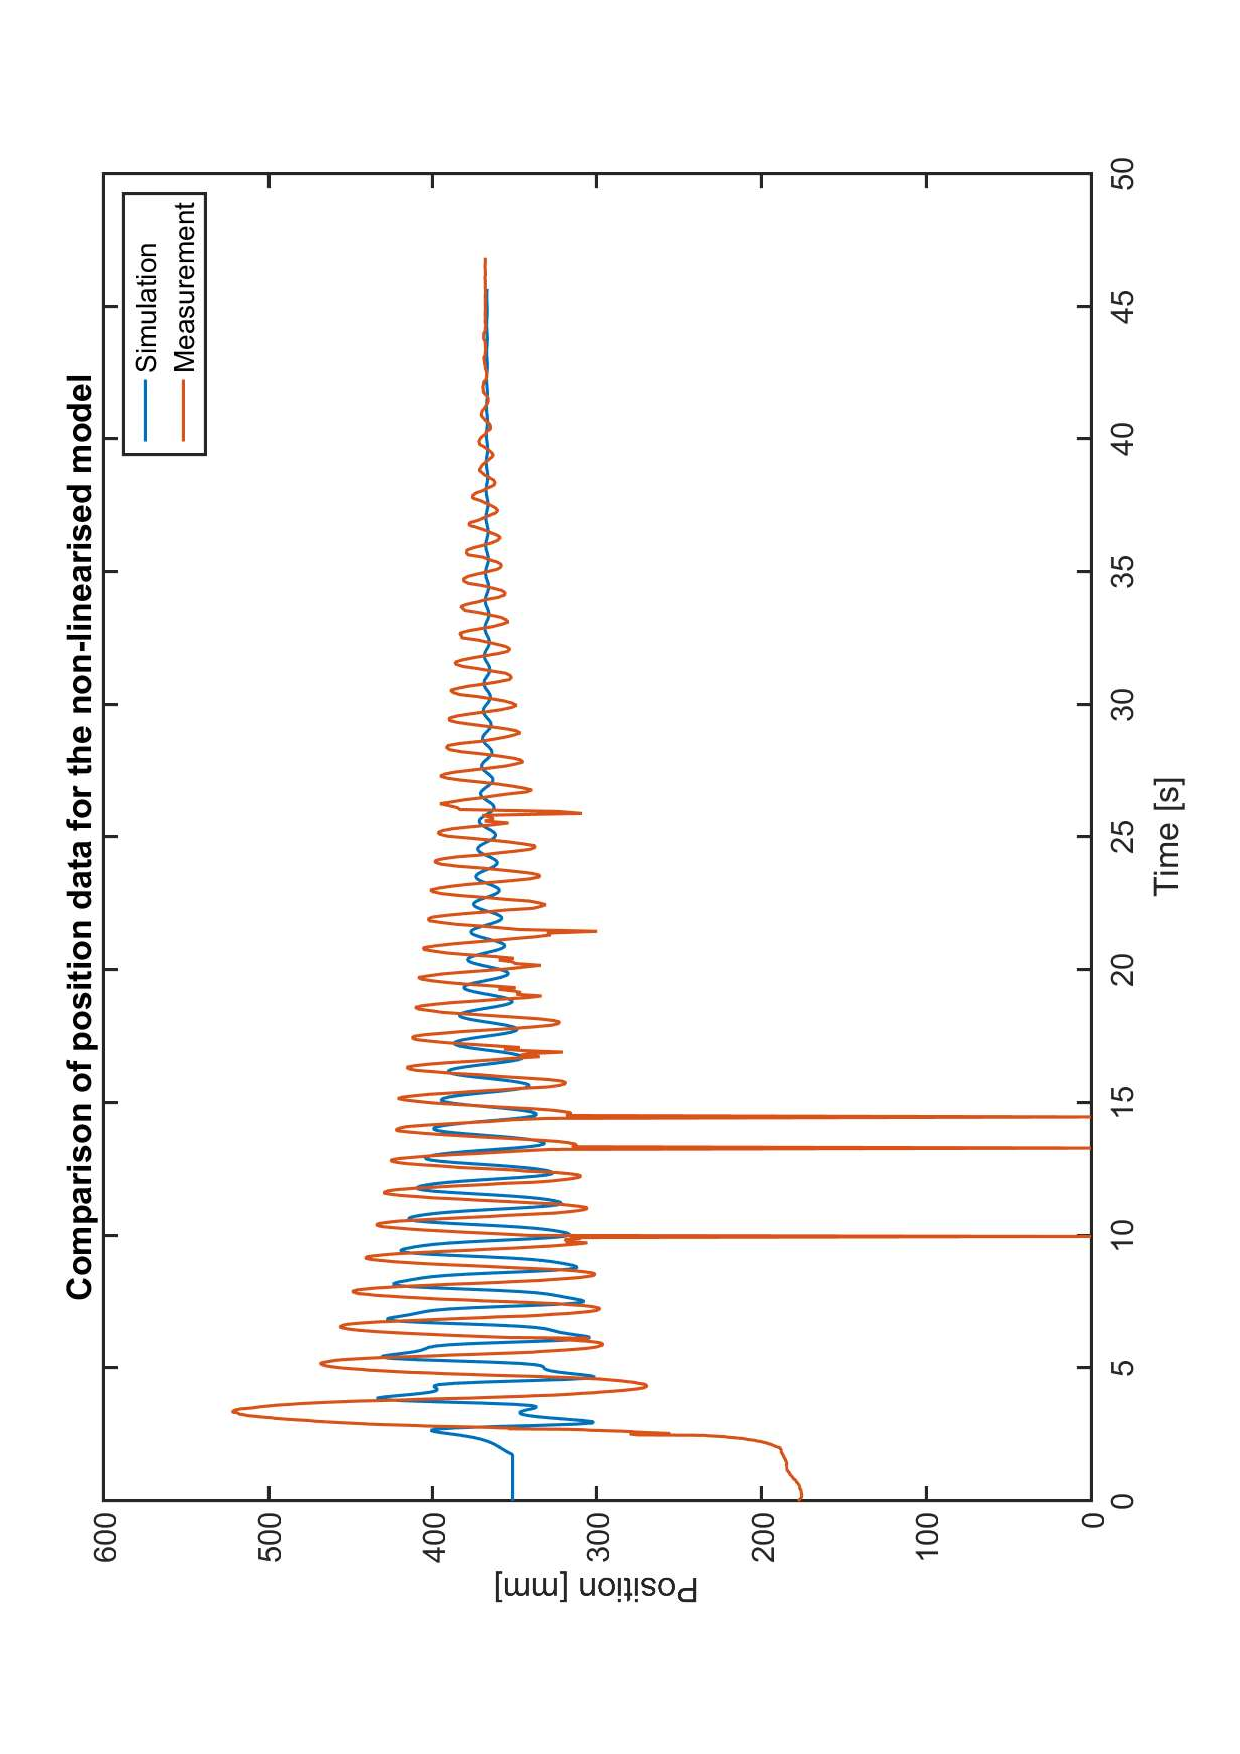
\includegraphics[height=\textwidth, angle = -90]{figures/SimMesInvPenPos.pdf}
\caption{Graph showing the entire impulse response of the cart position for the simulation and the test. The spikes are glitches.\label{fig:comPos}}
\end{figure}
